
\chapter{Diseño Experimental}

En este capítulo se explica a detalle el procedimiento experimental que se usó para determinar si las combinaciones de diferentes pesos dan lugar a resultados significativamente diferentes bajo pruebas estadísticas.  Primero comenzamos recordando las características principales del algoritmo de PFI-EMOA y cuáles van a ser las modificaciones que haremos para explorar diferentes configuraciones de parámetros de la escalarización de Tchebycheff. Después, en la Sección \ref{sec:Proc_exp}, detallaremos el procedimiento experimental seguido para obtener los resultados. La siguiente parte del capítulo, la Sección \ref{sec:Marco_Exp}, detalla todos los valores usados en los diferentes experimentos realizados; es decir, cuántas combinaciones de pesos se usaron, cuántas corridas por algoritmo, en cuáles problemas, con cuántos objetivos, con cuántas variables de decisión, el número de evaluaciones de los algoritmos evolutivos, etc. Finalmente se concluye el capítulo en la Sección \ref{sec:Resultados}, detallando los resultados obtenidos así como algunas visualizaciones de agrupaciones de datos interesantes. En particular, se muestra el desempeño (conteo de borda) de cada combinación de pesos, conforme se aumenta el número de dimensiones y para cada indicador diferente. 


Como mencionamos anteriormente en la Sección \ref{sec:PFI-EMOA}, el algoritmo en el que estamos basándonos \cite{PFI} emplea non-dominated sorting para decidir qué solución eliminar, sin embargo, cuando no existe un candidato obvio (porque hay varios en el último nivel) se recurre al uso de indicadores de calidad. En este algoritmo se ocupan dos indicadores que, sólo por el hecho de medir cosas diferentes, van a tener objetivos conflictivos; estos dos indicadores son IGD+ (revisado en la Sección \ref{sec:IGDp}) y la Energía-S de Riesz (revisada en la Sección \ref{sec:Energía-S}). 

El código usado para correr los experimentos y realizar las pruebas estadísticas se encuentra en el siguiente enlace \href{https://github.com/linear-regret/Tesis-LCD}{https://github.com/linear-regret/Tesis-LCD}


\section{Procedimiento de experimentación con diferentes pesos} \label{sec:Proc_exp}

Como se mencionó en la Sección \ref{sec:PFI-EMOA}, el algoritmo PFI-EMOA \cite{PFI} realiza una escalarización constante de los dos indicadores de calidad (Energía-S de Riesz e IGD+) para procurar que la solución no se estanque en convergencia ni tampoco en diversidad. La forma de la escalarización está dada por la función aumentada de Tchebycheff dada en la Ecuación \ref{eq:tchebychev}.

\begin{equation} \label{eq:ATCH2}
    \text{ATCH}_{\vec{w}}=\max_{i=0,1} \{w_ix_i\}+\alpha (x_0+x_1),  
\end{equation}

donde $x_0$ sería el IGD+ y $x_1$ la Energía-S de Riesz en PFI-EMOA. Además los pesos son tales que $ w_0+w_1=1$ de modo que podemos entender la razón entre ambos como la importancia que le estamos dando a cada indicador y por lo tanto a cada objetivo de ese indicador. Por ejemplo, si $w_0=0.4$ y $w_1=0.6$ podríamos decir, a grandes rasgos, que estamos dando 60\% de importancia a promover la diversidad y 40\% a promover la convergencia.   

En \cite{PFI} se usaron diferentes escalarizaciones constantes para los problemas dependiendo del número de objetivos del problema a resolver. En particular, se usó $\vec{w}=(\frac{1}{2},\frac{1}{2})$ para MOPs de dos y tres objetivos, mientras que para mayor número de objetivos se usó $\vec{w}=(\frac{9}{10},\frac{1}{10})$. Esta decisión se realizó porque cuando se incrementa el número de objetivos, el número de soluciones no dominadas incrementa exponencialmente (como se discutió en la Sección \ref{sec:QIs}). En este caso la Energía-S de Riesz puede recompensar soluciones con poco grado de convergencia. Al incrementar la prioridad que se le da a IGD+ se debería incrementar la presión de selección. 

En este trabajo se extendió el análisis de \cite{PFI} utilizando diferentes combinaciones de pesos en \eqref{eq:ATCH} con el objetivo de explorar qué sucede cuando se le da un peso distinto a cada uno de los indicadores. Para comparar los resultados se usaron conjuntos de problemas prueba usados frecuentemente en el campo de optimización multiobjetivo debido a que presentan diferentes retos para que los algoritmos encuentren una buena aproximación al frente de Pareto. En particular se usaron 2 familias de problemas estándar en el campo de optimización multiobjetivo. Estos problemas prueba tienen las propiedad de ser escalables (se pueden definir para cualquier número de objetivos) y además presentan diferentes retos para encontrar buenas aproximaciones al frente de Pareto. El primer conjunto de problemas tiene el prefijo WFG (Walking Fishing Group) y fue presentada por primera vez en \cite{hubandScalableMultiobjectiveTest2005}. El segundo conjunto de problemas  tiene el prefijo de DTLZ y  fue presentada por primera vez en \cite{debScalableMultiobjectiveOptimization2002}. El desempeño de cada configuración de cada algoritmo se evalúa en cada problema prueba usando indicadores de calidad de la solución que arroja cada uno de ellos. Por ejemplo, para la combinación de $w_0=0.4$ y $w_1=0.6$ se deja correr el algoritmo hasta que se cumple su condición de paro y a la población resultante se le calculan uno de los indicadores de calidad presentes en la tabla \ref{Tabla:QIs}. Como cada uno de estos indicadores expresa una característica diferente de la solución, el tomador de decisiones tendría que escoger cuál de estas cantidades quisiera optimizar para tener una solución más cercana a sus preferencias. Nuestro objetivo es mostrar que existen diferencias para algunos de estos indicadores medidos sobre las poblaciones finales de los diferentes algoritmos (combinaciones de peso) de modo que podemos escoger una combinación específica de pesos si buscamos maximizar un indicador en particular.  
Así, para cada problema de prueba dado en la Tabla \ref{Tabla:problema_prueba}, se siguieron los pasos que se explican a continuación:

% TODO: Comenzar la discusión diciendo que se va a llamar algoritmos distintos a cada configuración de pesos.
% TODO: Poner el ejemplo desde el planteamiento de un problema y cómo se iría explorando la solución. 
\begin{enumerate}
    \item Se divide el espacio de pesos en 10 igualmente espaciados dados por 
    \begin{align} \label{eq:pesosw}
        \vec{w} \in \big\{ &(0.001,0.999),(0.1,0.9),(0.2,0.8),(0.3,0.7),(0.4,0.6) \nonumber\\
         &(0.5,0.5),(0.6,0.4),(0.7,0.3),(0.8,0.2),(0.9,0.1),(0.999,0.001) \big\}.
    \end{align}
    Siendo los primeros valores aquellos donde se toma más en cuenta el indicador de uniformidad (al ser menor $w_1$) y los últimos valores donde se prioriza el indicador de convergencia \footnote{Cabe destacar que los extremos de este conjunto $(0,1),(1,0)$ no se tomaron como tal porque daban lugar a los mismos resultados. Esto se discute en la siguiente sección.}.
    \item Para cada combinación de pesos en la Ecuación \ref{eq:pesosw}, se procede a ejecutar el algoritmo de PFI-EMOA, explicado en la Sección \ref{sec:PFI-EMOA}, con un número $f_{eval}=50,000$ de evaluaciones de la función de aptitud, es decir, $50000$  generaciones.
    \
    \item Cada una de las combinaciones de pesos se ejecuta un número $n_{runs}=10$ de veces con distintas configuraciones aleatorias de su población inicial. La inicialización está controlada por un conjunto de semillas fijas\footnote{El conjunto de semillas usadas se encuentra en el Apéndice \ref{sec:Apendice_semilla}.}, de esta forma se puede garantizar la reproducibilidad de los resultados.  

    \item Después, se procede al cálculo de los indicadores de calidad de cada población. Los indicadores que se trataron en este trabajo se pueden ver en la Tabla \ref{Tabla:QIs} que muestra cada uno de los indicadores junto su categoría principal de las revisadas en la Figura \ref{fig:carac_deseables_aprox}.
    \item Finalmente, después de realizar el cálculo de todos los indicadores de calidad, se realiza un análisis estadístico para determinar si tiene algún efecto el cambiar los pesos de la escalarización y, si lo tiene, cuál es el mejor y en qué medida. Esto se realiza por medio de las pruebas estadísticas de Friedman (para la parte de ver diferencias) y usando Wilcoxon como análisis post-hoc para ver cuáles de ellas son mejores a las otras.     
\end{enumerate}


\begin{table}[H]
    \centering
    \begin{tabular}{|c|c|}
    \textbf{Indicador} & \textbf{Categoría principal} \\ \hline
    \hyperref[sec:IGDp]{IGD+}      & Convergencia                  \\
    \hyperref[sec:R2]{R2}         & Convergencia                  \\
    \hyperref[sec:Energía-S]{Energía-S}    & Diversidad                   \\
    \hyperref[sec:Epsilonp]{$\epsilon +$}       & Convergencia                  \\
    \hyperref[sec:IGD]{IGD}       & Convergencia                  \\
    \hyperref[sec:SPD]{SPD}        & Diversidad                   \\
    \hyperref[sec:HV]{Hipervolumen}        & Convergencia                 
    \end{tabular}
    \caption[QI para cada problema]{Indicadores de Calidad usados para cada uno de los problemas prueba. Para cada indicador se muestra la categoría principal en la que cae de las detalladas en la Sección \ref{sec:QIs_tax}. Cada indicador tiene un hipervínculo a la Sección que lo explica.}
    \label{Tabla:QIs}
\end{table}


A continuación se muestra la Tabla \ref{Tabla:problema_prueba} donde viene información relevante acerca de todos los problemas de prueba considerados, así como algunas características de su frente de Pareto. Cabe destacar que el número de variables de decisión está dado, como se menciona en \cite{PFI}, por $n=24+2(m-2)$, donde $m$ es el número de objetivos. Los problemas WFG también cuentan con parámetros relacionados a su posición, estos también están dados en términos del número de objetivos por $k=2(m-1)$. Para los problemas de la familia DTLZ, tenemos que el número de variables está dado por $n=m+l-1$, con $l=5$ para DTLZ1, $l=10$ para DTLZ2-DTLZ6 y $l=20$ para DTLZ7.

\begin{table}[H]
    \centering
    \resizebox{\textwidth}{!}{%
        \begin{tabular}{|l|l|l|l|l|l|l|}
        \textbf{Problema} & \textbf{Número de objetivos} & \textbf{Número de variables de decisión} & \textbf{Separabilidad}                                                           & \textbf{Frontalidad}                                                             & \textbf{Geometría}                                                         & \textbf{Sesgo}                                              \\ \hline
        DTLZ1             & 2,3,4,5,6,7                  & 6,7,8,9,10,11                            & separable                                                                        & multifrontal                                                                     & lineal                                                                     & no                                                          \\
        DTLZ2             & 2,3,4,5,6,7                  & 12,13,14,15,16                           & separable                                                                        & unifrontal                                                                       & cóncavo                                                                    & no                                                          \\
        \textbf{DTLZ3}    & 2,3,4,5,6,7                  & 12,13,14,15,16                           & separable                                                                        & multifrontal                                                                     & cóncavo                                                                    & no                                                          \\
        DTLZ4             & 2,3,4,5,6,7                  & 12,13,14,15,16                           & separable                                                                        & unifrontal                                                                       & cóncavo                                                                    & polinomial                                                  \\
        DTLZ5             & 2,3,4,5,6,7                  & 12,13,14,15,16                           & desconocido                                                                      & unifrontal                                                                       & degenerado                                                                 & dependiente de los parámetros                               \\
        DTLZ6             & 2,3,4,5,6,7                  & 12,13,14,15,16                           & desconocido                                                                      & unifrontal                                                                       & degenerado                                                                 & dependiente de los parámetros                               \\
        DTLZ7             & 2,3,4,5,6,7                  & 21,22,23,24,25,26                        & \begin{tabular}[c]{@{}l@{}}$f_{1:m-1}$ no aplica,\\ $f_m$ separable\end{tabular} & \begin{tabular}[c]{@{}l@{}}$f_{1:m-1}$ unimodal,\\ $f_m$ multimodal\end{tabular} & \begin{tabular}[c]{@{}l@{}}desconectado,\\ mixto\end{tabular}              & no                                                          \\
        WFG1              & 2,3,4,5,6,7                  & 24,26,28,30,32,34                        & separable                                                                        & unifrontal                                                                       & \begin{tabular}[c]{@{}l@{}}$f_{1:m-1}$ convexo,\\ $f_m$ mixto\end{tabular} & \begin{tabular}[c]{@{}l@{}}polinomial,\\ plano\end{tabular} \\
        WFG2              & 2,3,4,5,6,7                  & 24,26,28,30,32,34                        & no separable                                                                     & \begin{tabular}[c]{@{}l@{}}$f_{1:m-1}$ unimodal,\\ $f_m$ multimodal\end{tabular} & \begin{tabular}[c]{@{}l@{}}conexo,\\ desconectado\end{tabular}             & no                                                          \\
        WFG3              & 2,3,4,5,6,7                  & 24,26,28,30,32,34                        & no separable                                                                     & unifrontal                                                                       & \begin{tabular}[c]{@{}l@{}}lineal,\\ degenerado\end{tabular}               & no                                                          \\
        WFG4              & 2,3,4,5,6,7                  & 24,26,28,30,32,34                        & separable                                                                        & multifrontal                                                                     & cóncavo                                                                    & no                                                          \\
        WFG5              & 2,3,4,5,6,7                  & 24,26,28,30,32,34                        & separable                                                                        & deceptivo                                                                        & cóncavo                                                                    & no                                                          \\
        WFG6              & 2,3,4,5,6,7                  & 24,26,28,30,32,34                        & no separable                                                                     & unifrontal                                                                       & cóncavo                                                                    & no                                                          \\
        WFG7              & 2,3,4,5,6,7                  & 24,26,28,30,32,34                        & separable                                                                        & unifrontal                                                                       & cóncavo                                                                    & dependiente de los parámetros                               \\
        WFG8              & 2,3,4,5,6,7                  & 24,26,28,30,32,34                        & no separable                                                                     & unifrontal                                                                       & cóncavo                                                                    & dependiente de los parámetros                               \\
        WFG9              & 2,3,4,5,6,7                  & 24,26,28,30,32,34                        & no separable                                                                     & \begin{tabular}[c]{@{}l@{}}multifrontal,\\ deceptivo\end{tabular}                & cóncao                                                                     & dependiente de los parámetros                              
        \end{tabular}
    }
    \caption[Problemas prueba usados]{Problemas pruebas usados así como el total de variables objetivo $m$, de decisión,  y algunas características de su frente de Pareto.}
    \label{Tabla:problema_prueba}
    \end{table}

En estas dos últimas Tablas las características del frente de Pareto se refieren a lo siguiente:

\begin{itemize}
    \item \textbf{Separabilidad}: Un frente de Pareto es ``separable'' cuando las soluciones pueden clasificarse o separarse fácilmente en base a sus objetivos. Esto generalmente facilita la optimización, ya que puedes optimizar cada objetivo por separado y luego combinarlos.
    
    \item \textbf{Frontalidad}: Se refiere a la existencia de múltiples ``capas'' o ``frentes'' en el conjunto de soluciones no dominadas. En algunos casos, especialmente en problemas complejos, puede haber varias capas de soluciones que son no dominadas entre sí pero que son dominadas por soluciones en un frente superior.
    
    \item \textbf{Geometría}: Encontramos las siguientes categorías \begin{itemize}
        \item    Un frente de Pareto ``lineal'' sugiere que existe una relación lineal entre los objetivos en el frente óptimo. Esto puede simplificar mucho el problema de optimización, ya que las técnicas lineales son computacionalmente menos exigentes.
        
        \item \textbf{Cóncavo}: Un frente de Pareto ``cóncavo'' tiene una forma que se hunde hacia adentro, sugiriendo que hay una especie de ``compromiso'' entre los objetivos. En estos casos, mejorar en un objetivo puede llevar a un deterioro significativo en otro.
        
        \item \textbf{Degenerado}: Un frente ``degenerado'' contiene soluciones que son técnicamente no dominadas pero que son muy similares o idénticas en términos prácticos. Esto puede suceder debido a la discretización, errores numéricos o la naturaleza del problema de optimización. Por ejemplo que la dimensión del frente de Pareto no sea una menos que la del espacio de objetivos sino menor. 
        
        \item \textbf{Desconectado}: Un frente ``desconectado'' consiste en clústeres de soluciones no dominadas que están separadas entre sí. Esto podría implicar que hay ``saltos'' en el espacio de soluciones que son difíciles de cruzar mediante optimización continua.
        
        \item \textbf{Mixto}: Un frente ``mixto'' podría tener una combinación de varias de las características anteriores. Por ejemplo, podría ser en parte lineal y en parte cóncavo, o podría tener segmentos separables y no separables.
    \end{itemize}
    \item \textbf{Sesgo}: Que tanto se encuentra en la dirección de algún objetivo preferencialmente. 
\end{itemize}



\section{Marco Experimental} \label{sec:Marco_Exp}


Los parámetros de la Tabla \ref{Tabla:problema_prueba} nos ayudan a ejecutar el algoritmo con cada combinación de pesos. Sin embargo, los algoritmos evolutivos tienen un elemento aleatorio en cada una de sus etapas, como revisamos en la Sección \ref{sec:AE}, así que no podemos comparar simplemente la salida de una ejecución de dos algoritmos. Así, hacemos 10 ejecuciones de cada algoritmo, estas ejecuciones se realizan de modo que cada una de ellas tenga sus elementos aleatorios controlado por una semilla diferente; esto último nos garantiza reproducibilidad de los mismos resultados. 

Después de hacer las 10 ejecuciones para cada uno de los problemas con cada conjunto de pesos tenemos una población final por cada ejecución. De estas poblaciones nos interesa comparar su desempeño en los indicadores de la Tabla \ref{Tabla:QIs}. Entonces, para una combinación de pesos $\vec{w}_i$, de los valores disponibles en \eqref{eq:pesosw}, un problema prueba de los encontrados en la Tabla \ref{Tabla:problema_prueba}, con un número de objetivos específico, se ejecuta el algoritmo PFI-EMOA 10 veces con sus semillas respectivas. Así, se obtienen 10 conjuntos de soluciones como la que se observa en la Figura \ref{fig:aproximacion}. De estas 10 poblaciones se calcula cada valor de los indicadores de la Tabla \ref{Tabla:QIs} y entonces se obtiene un conjunto de valores de indicadores que se puede visualizar, por ejemplo, a través de un boxplot como el de la Figura \ref{fig:box}.

Los indicadores de calidad fueron calculados usando el programa de \emph{Assessment} utilizado en el Artículo \cite{PFI}. Al terminar de calcular todos los indicadores de calidad para todas las corridas para todos los problemas prueba en todas las dimensiones tenemos una tabla de valores de indicadores que tiene una cardinalidad dada por la Ecuación \ref{eq:cardinalidad}. 

\begin{align} \label{eq:cardinalidad}
    |\text{Valores de indicadores}|&=N_{ejec}*N_{indicadores}*N_{problemas}*N_{dimensiones}*N_{pesos} \nonumber\\
    &=10*7*16*6*11 \nonumber \\
    &=73920. 
\end{align}



\section{Resultados} \label{sec:Resultados}

En esta sección se muestran visualizaciones que se obtuvieron para cada problema y para cada indicador. Como el número de valores de indicadores es muy grande, como vimos en la Ecuación \ref{eq:cardinalidad}, se dejan las figuras completas en el Apéndice A.

Para cada problema y con el objetivo de poder detectar errores en el código y casos interesantes, se realizaron las siguientes visualizaciones:

\begin{itemize}
    % TODO: Poner primero una gráfica de la forma del DTLZ3 y luego de las aproximaciones
    \item Una función para visualizar la aproximación al frente de Pareto. Como podemos ver en las Figura \ref{fig:aproximacion} \footnote{Cuando el número de objetivos es mayor a 3 se usa una malla de proyecciones sobre cada uno de los objetivos} donde se grafica cada punto del conjunto de soluciones para el problema de DTLZ3 en 3 objetivos para todos los pesos, es decir, cada eje corresponde a un objetivo distinto . En 3 dimensiones, podemos visualizar la aproximación al frente de Pareto en todos los objetivos. En el caso de la Figura \ref{fig:aproximacion} vemos una malla de aproximaciones para los diferentes pesos. Comenzando en la esquina superior izquierda con $\vec{w}=(0.001,0.999)$ y continuando hacia la derecha hasta llegar al $\vec{w}=(0.999,0.001)$. Como podemos ver, casi todos tienen una configuración similar con la excepción de $\vec{w}=(0.1,0.9)$. Cabe destacar que esta malla fue generada con el algoritmo que usa como indicador de convergencia a IGD+.
    \item Además se produce una gráfica de coordenadas paralelas para ayudar a visualizar casos de mayores dimensiones como en la Figura \ref{fig:PCP}. Estas funciones se pueden tomar como una por cada ejecución, sin embargo para tomar una muestra que sea representativa del desempeño de cada configuración de algoritmos, tomamos aquella ejecución que está en la mediana del desempeño según el indicador de hipervolumen. Este tipo de visualizaciones son mucho más útiles cuando el número de objetivos es mayor a 3. Podemos ver cómo la misma combinación de la Figura \ref{fig:aproximacion} es la que se ve distinta por un outlier en la dirección $f_2$ que llega casi al valor de 2 del peso $w_0=0.1$. Al igual que en la imagen anterior, para esta visualización se usó el algoritmo que tiene a IGD+ como indicador de convergencia.
    \item Una función para visualizar un boxplot por cada problema y por cada indicador. Esto tiene un resumen de toda la información de cada una de las 10 ejecuciones para cada combinación de pesos, como en la Figura \ref{fig:box}.  Vemos en esa figura que hay variaciones entre los diferentes valores de $w_0$ aunque para tener algún tipo de confiabilidad tenemos que hacer las pruebas estadísticas de la siguiente sección. En esta figura se muestran los dos algoritmos, tanto con R2 como con IGD+ y podemos observar que a grandes rasgos se comportan similar, pero hay menor variación para R2. Esta observación la haremos más puntual más adelante.
    \item Una tabla con toda la información de cada valor del indicador.
\end{itemize}


\begin{figure} [H]
    \centering
    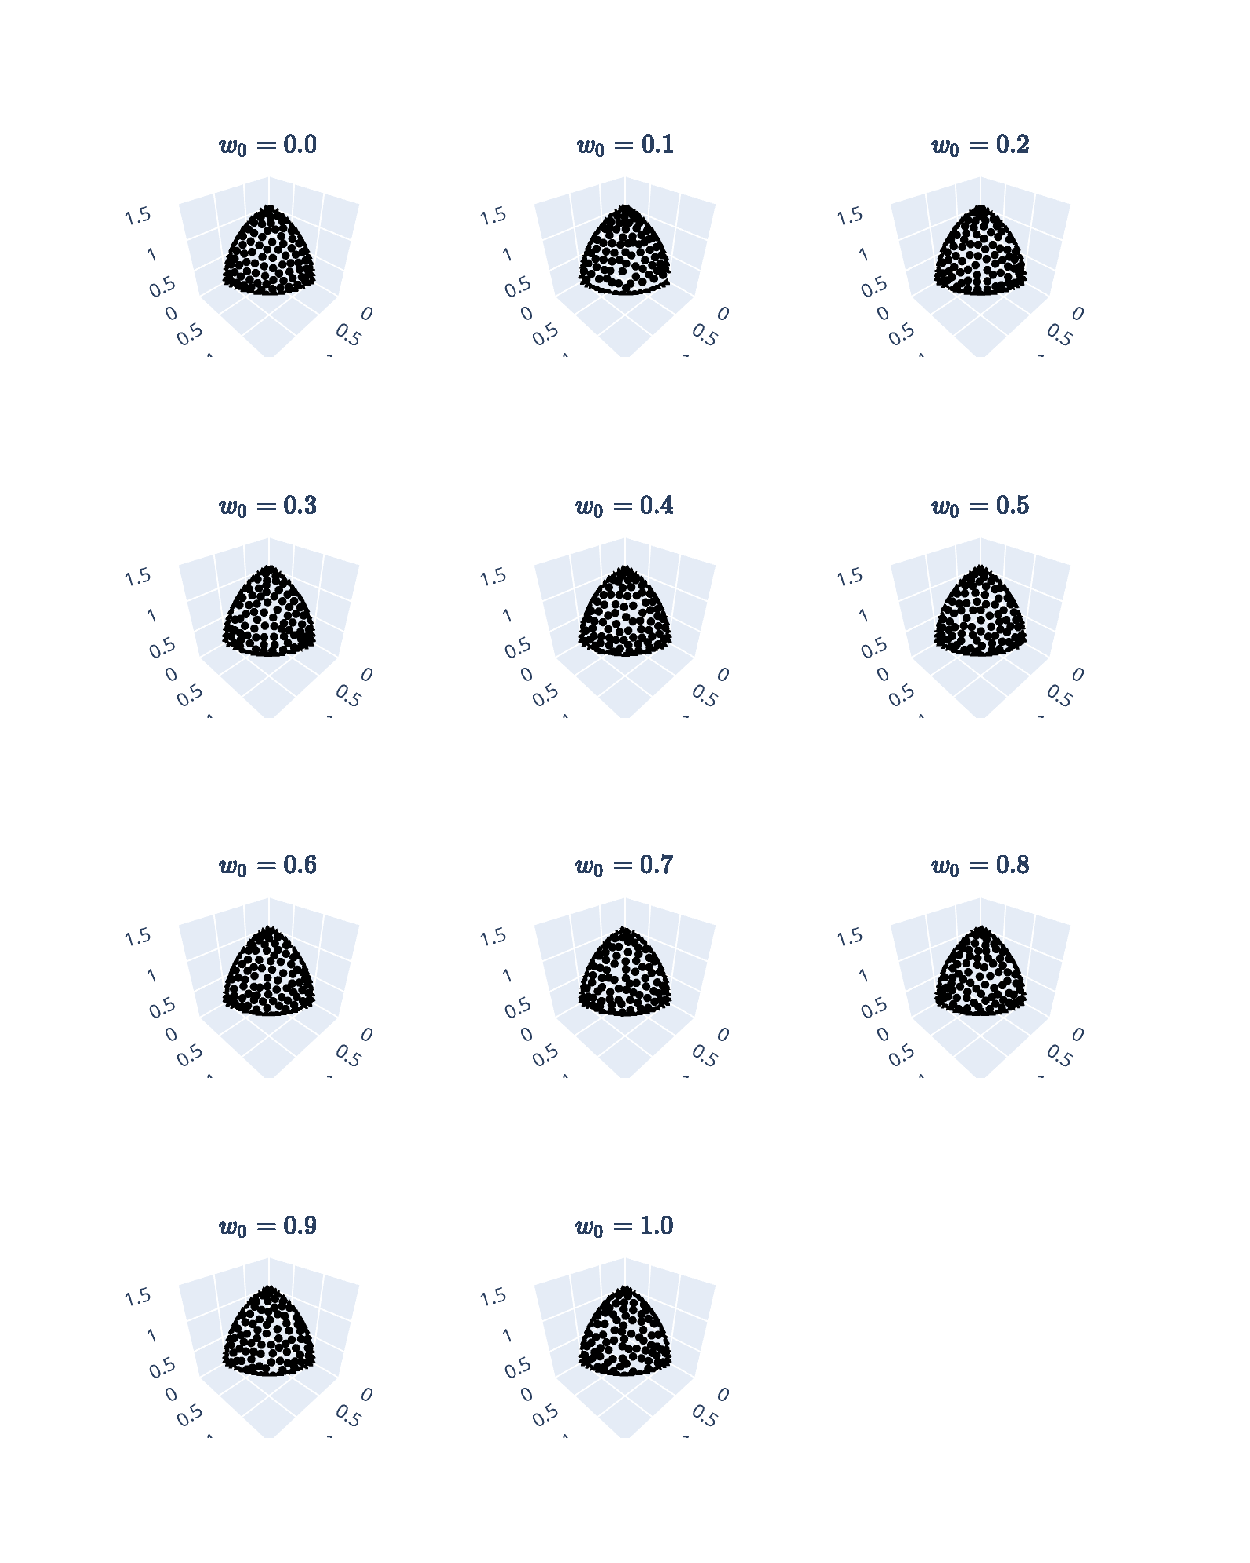
\includegraphics[width=\textwidth]{Figuras/DTLZ3_obj_3_alg_IGD+_indmed_HV_malla.pdf}
    \caption[Aproximación 3D al PF]{Malla de conjunto de aproximaciones para diferentes pesos para DTLZ3 en 3 objetivos.}
    \label{fig:aproximacion}
\end{figure}

\begin{figure} [H]
    \centering
    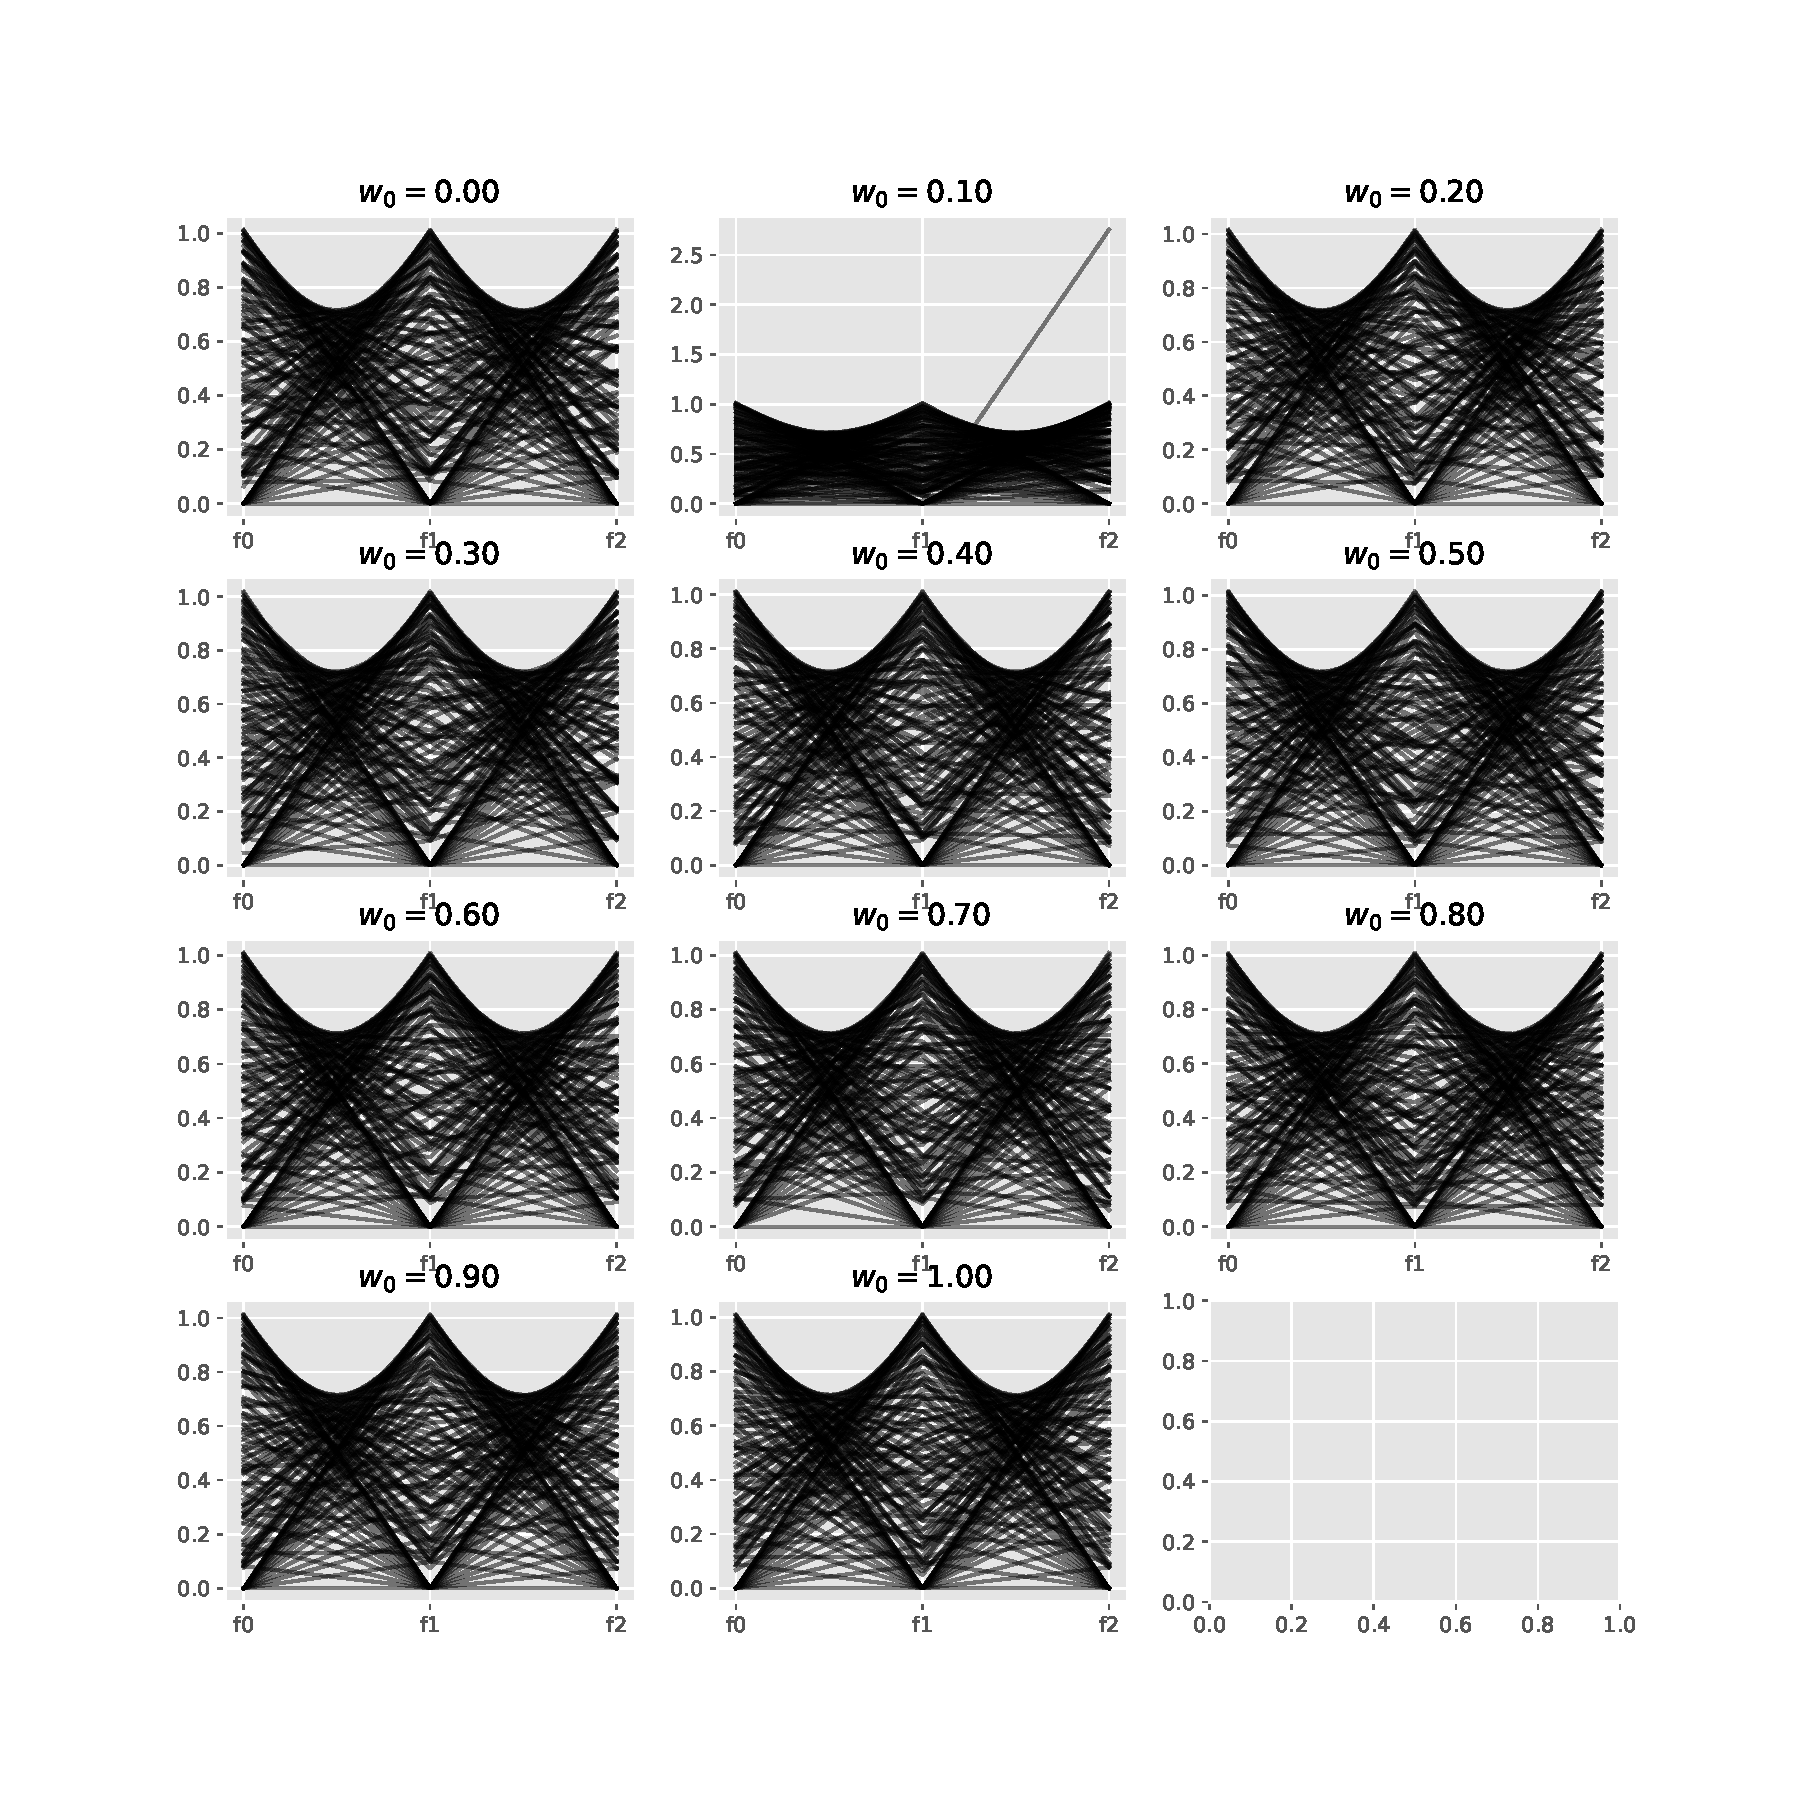
\includegraphics[width=\textwidth]{Figuras/DTLZ3_obj_3_alg_IGD+_indmed_HV_malla._PCP.pdf}
    \caption[Malla de PCP  de aproximaciones al PF.]{Malla de PCP para DTLZ3 en 3 objetivos.}
    \label{fig:PCP}
\end{figure}



\begin{figure} [H]
    \centering
    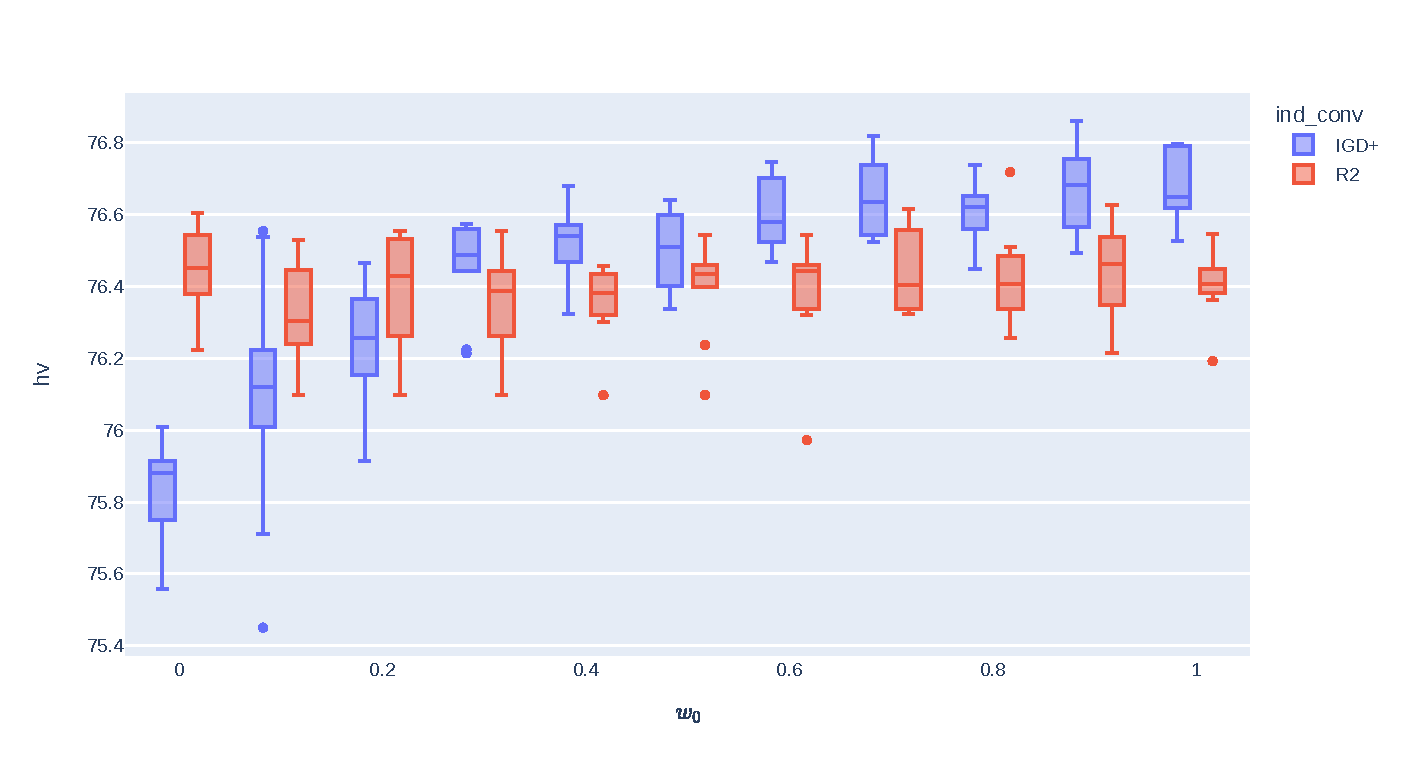
\includegraphics[width=\textwidth]{Figuras/WFG4_3obj_HV.pdf}
    \caption[Boxplot WFG4 3 Objetivos HV.]{Boxplot WFG4 con 3 objetivos con el indicador de Hipervolumen. La variable DE\_ind\_conv indica qué indicador de calidad se usó en la combinación de Tchebycheff de la Ecuación \eqref{eq:tchebychev}.}
    \label{fig:box}
\end{figure}




\subsection{Pruebas Estadísticas}

Como se explicó en la Sección \ref{sec:pruebas_estadisticas}, para saber si un algoritmo tiene un desempeño diferente en un indicador dado usamos la prueba de Friedman \ref{sec:Friedman} implementada en la librería de \href{https://docs.scipy.org/doc/scipy/reference/stats.html}{scipy.stats}. En total obtenemos que un $25.37\%$ de los problemas presentan una diferencia significativa, es decir, se rechaza la hipótesis nula.

Algunos resultados agregados de este procedimiento se pueden ver en las siguientes dos Figuras. En la primera imagen de la Figura \ref{fig:Fr_dim_IGDp} se usó el algoritmo con IGD+ mientras que en la Figura \ref{fig:Fr_dim_R2} R2. Podemos ver que en R2 existen mucho menos diferencias de acuerdo a Friedman.   La prueba sólo indica si hay una diferencia significativa entre al menos una de las observaciones con el resto. Vemos que importa mucho ajustar los pesos para indicadores como IGD+, HV, IGD y en menor medida para Energía-S. Vemos que para dos dimensiones parece importar menos que pesos escojamos para el desempeño de todos los indicadores. 

\begin{figure}[H]
    \centering
    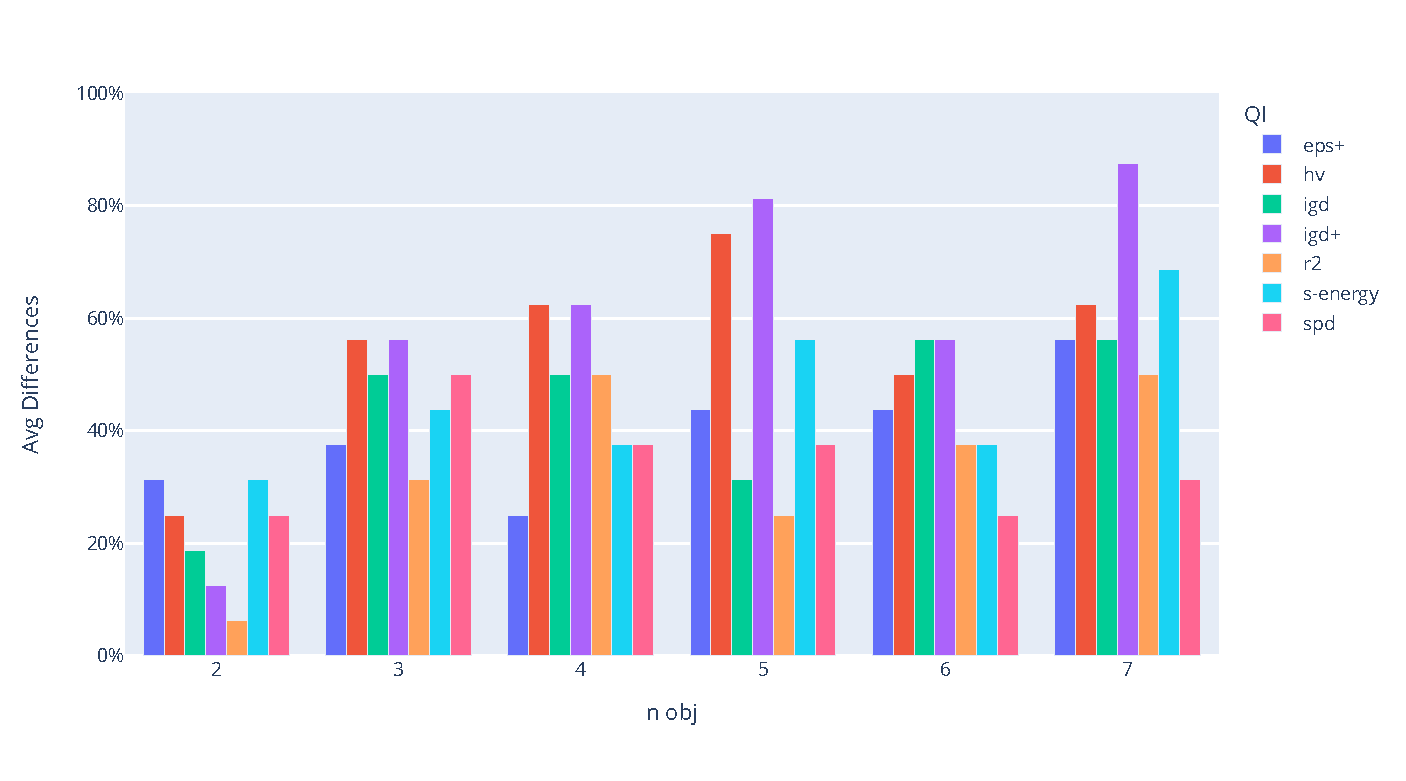
\includegraphics[width=\textwidth]{Figuras/Friedman_obj_indconv_IGD+.pdf}
    \caption[Friedman IGD+]{Diferencias cuando el indicador de convergencia de ATCH es IGD+.}
    \label{fig:Fr_dim_IGDp}
\end{figure}

\begin{figure}[H]
    \centering
    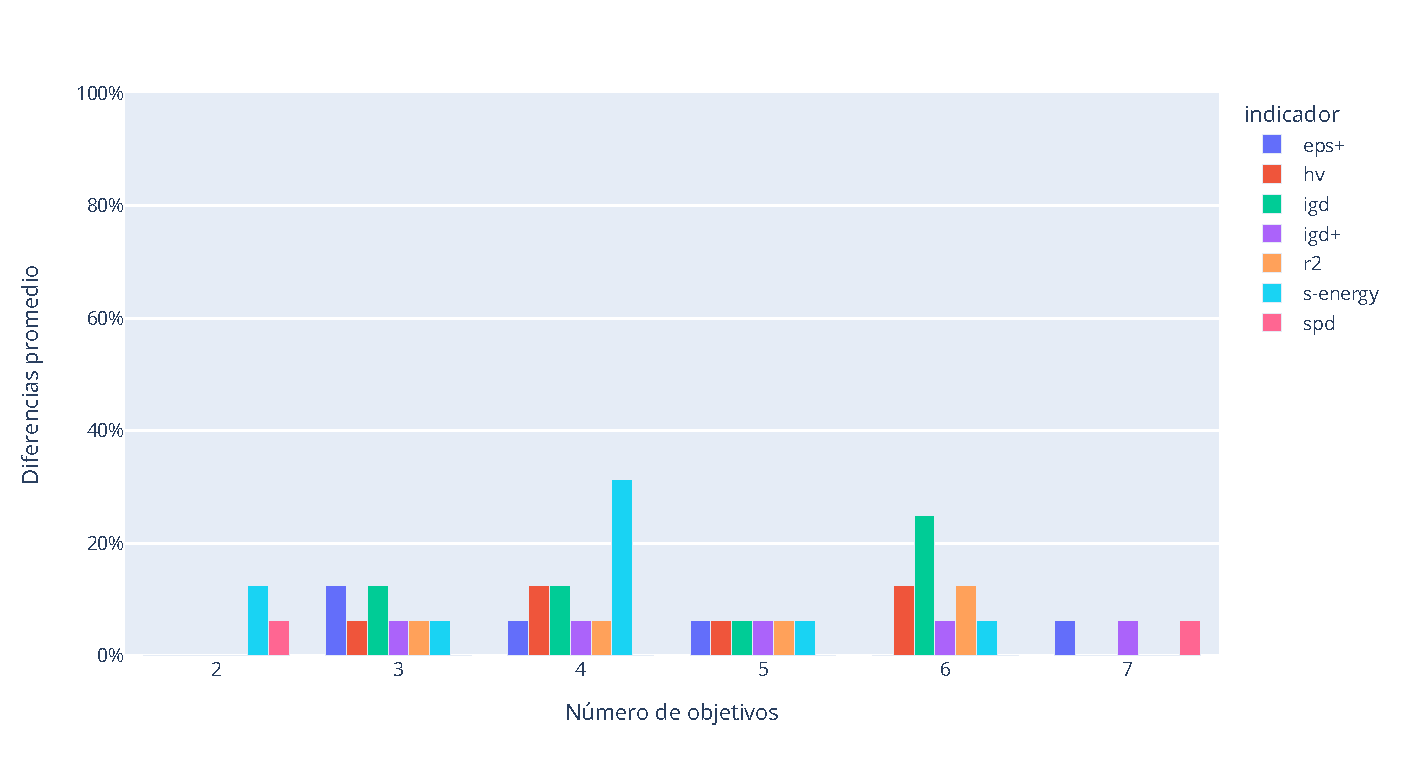
\includegraphics[width=\textwidth]{Figuras/Friedman_obj_indconv_R2.pdf}
    \caption[Friedman R2]{Diferencias cuando el indicador de convergencia de ATCH es R2.}
    \label{fig:Fr_dim_R2}
\end{figure}


De la misma forma, en la Figura \ref{fig:Friedman_Diferencia_por_categoria_IGD} hacemos una agregación por categoría de Indicador para el caso donde el indicador de convergencia en el estimador de densidad es IGD+, mientras que para R2 tenemos la Figura \ref{fig:Friedman_Diferencia_por_categoria_R2}. Nuevamente observamos como el algoritmo de IGD+ presenta más sensibilidad a la elección de parámetros. Basándonos en la clasificación de la Tabla \ref{Tabla:QIs} separamos los problemas para ver si se va volviendo más importante la selección de $w_0$ conforme aumentamos la dimensión. Vemos que el número de objetivos parece importar un poco más para los indicadores convergencia y obtenemos el mismo resultado de la figura anterior, en el sentido en el que para 2 objetivos no parece importar mucho la escalarización que usemos.

\begin{figure}[H]
    \centering
    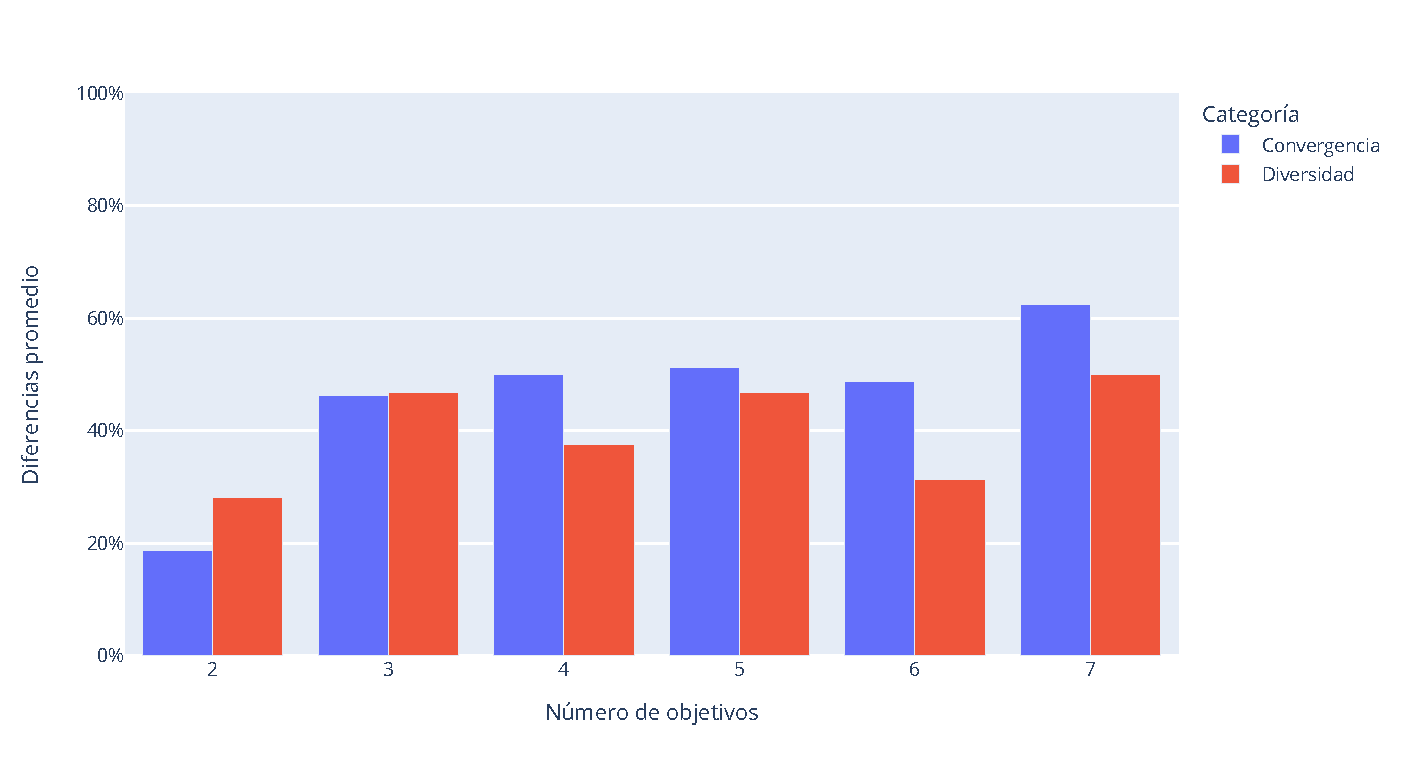
\includegraphics[width=\textwidth]{Figuras/Friedman_Diferencia_por_categoria_IGD+.pdf}
    \caption[Friedman por categoría para IGD+.]{Friedman por categoría de indicadores de acuerdo a la Tabla \ref{Tabla:QIs} cuando el indicador de convergencia de ATCH es IGD+.}
    \label{fig:Friedman_Diferencia_por_categoria_IGD}
\end{figure}

\begin{figure}[H]
    \centering
    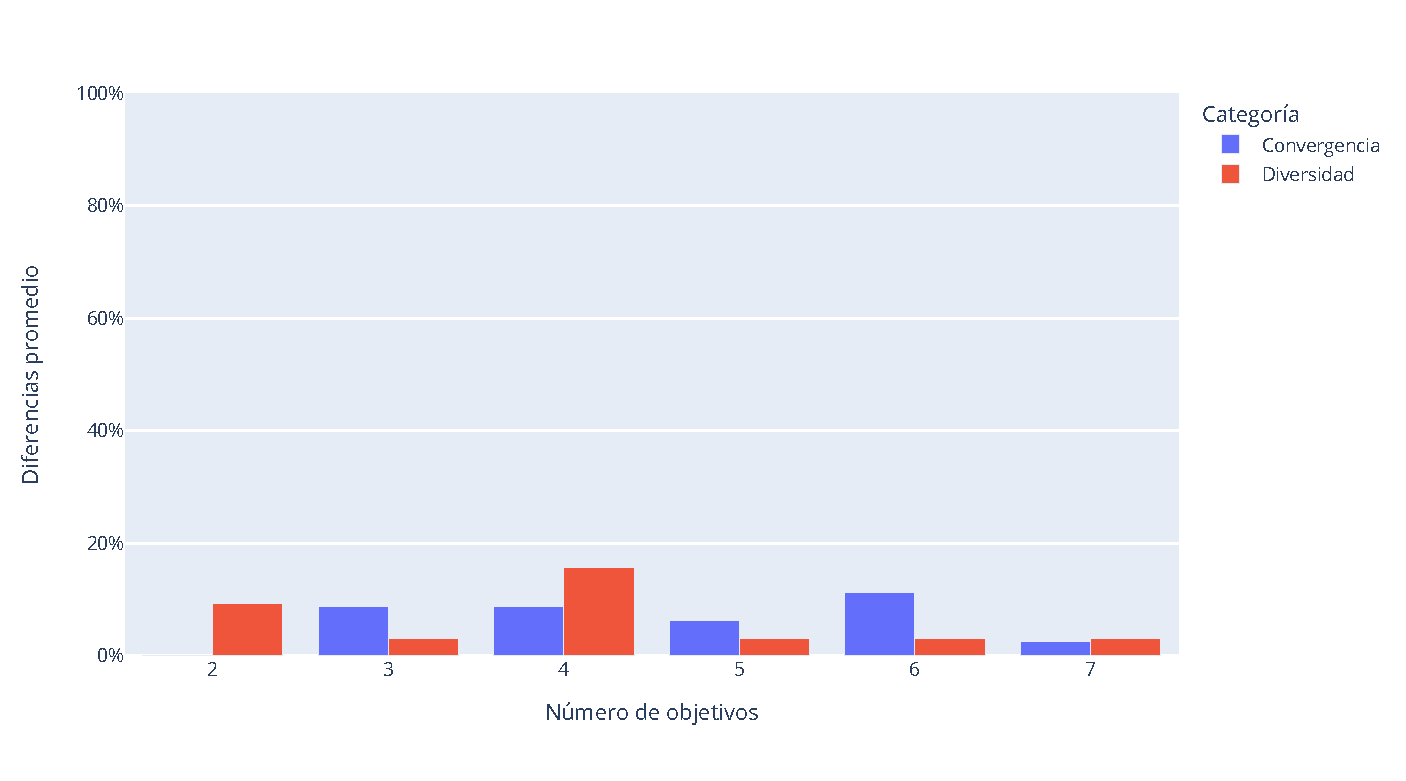
\includegraphics[width=\textwidth]{Figuras/Friedman_Diferencia_por_categoria_R2.pdf}
    \caption[Friedman por categoría para R2.]{Friedman por categoría de que indicador usamos de acuerdo a la Tabla \ref{Tabla:QIs} cuando el indicador de convergencia de ATCH es R2.}
    \label{fig:Friedman_Diferencia_por_categoria_R2}
\end{figure}


\section*{Comparación uno a uno}
Para saber si un algoritmo $A_1$ tiene un mejor desempeño que otro algoritmo $A_2$ usaremos la prueba de Wilcoxon que revisamos en la Sección \ref{sec:Wilcoxon}. Así, comparando con los diferentes valores de los pesos para la escalarización, obtenemos una Tabla como la de la Figura \ref{fig:heat}. En esta figura la hipótesis nula es que el peso del renglón no es mejor que el de la columna. Hay que recordar que algunos indicadores son maximizados y otros minimizados así que hay que escoger la dirección correcta en la implementación de scipy.stats. Es de esperarse que los valores altos de $w_0$ den como resultado un mejor hipervolumen pues es para estos que se favorece el indicador de convergencia.

\begin{figure} [H]
    \centering
    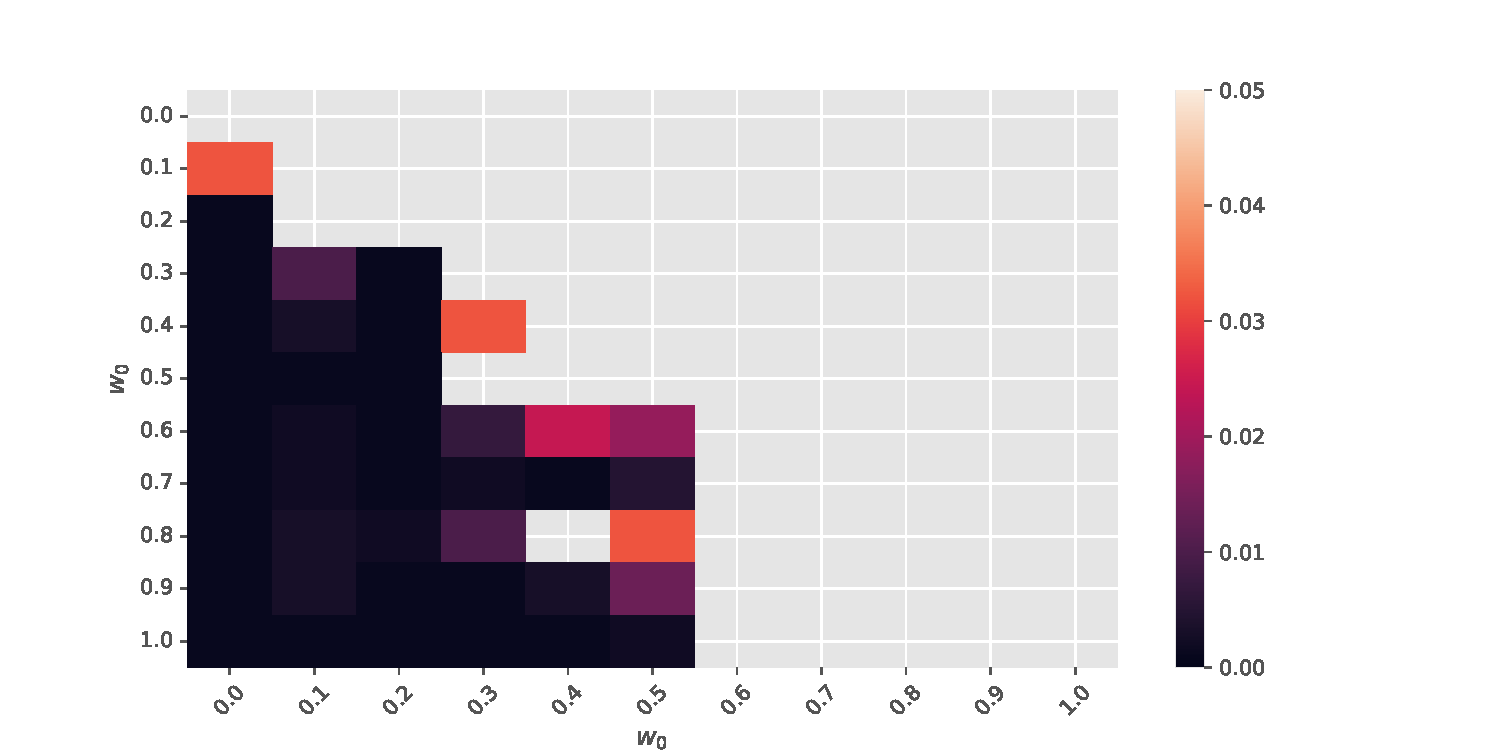
\includegraphics[width=0.8\textwidth]{Figuras/Heatmap_WFG4_obj3_hv_indconv_IGD+.pdf}
    \caption[Heatmap Wilcoxon]{Vemos un mapa de calor con el valor de la prueba $p$ para la prueba de Wilcoxon. }
    \label{fig:heat}
\end{figure}

Podemos obtener el número de las victorias de cada uno de los valores si simplemente contamos cuántas pruebas resultan ser significativamente mejores. Es decir, contando cuántos cuadros hay en la Figura en \ref{fig:heat} están coloreados para una columna dada. A esta manera de establecer ganadores se le conoce como conteo de borda y lo podemos visualizar en la Figura \ref{fig:borda_problema}.

\begin{figure}[H]
    \centering
    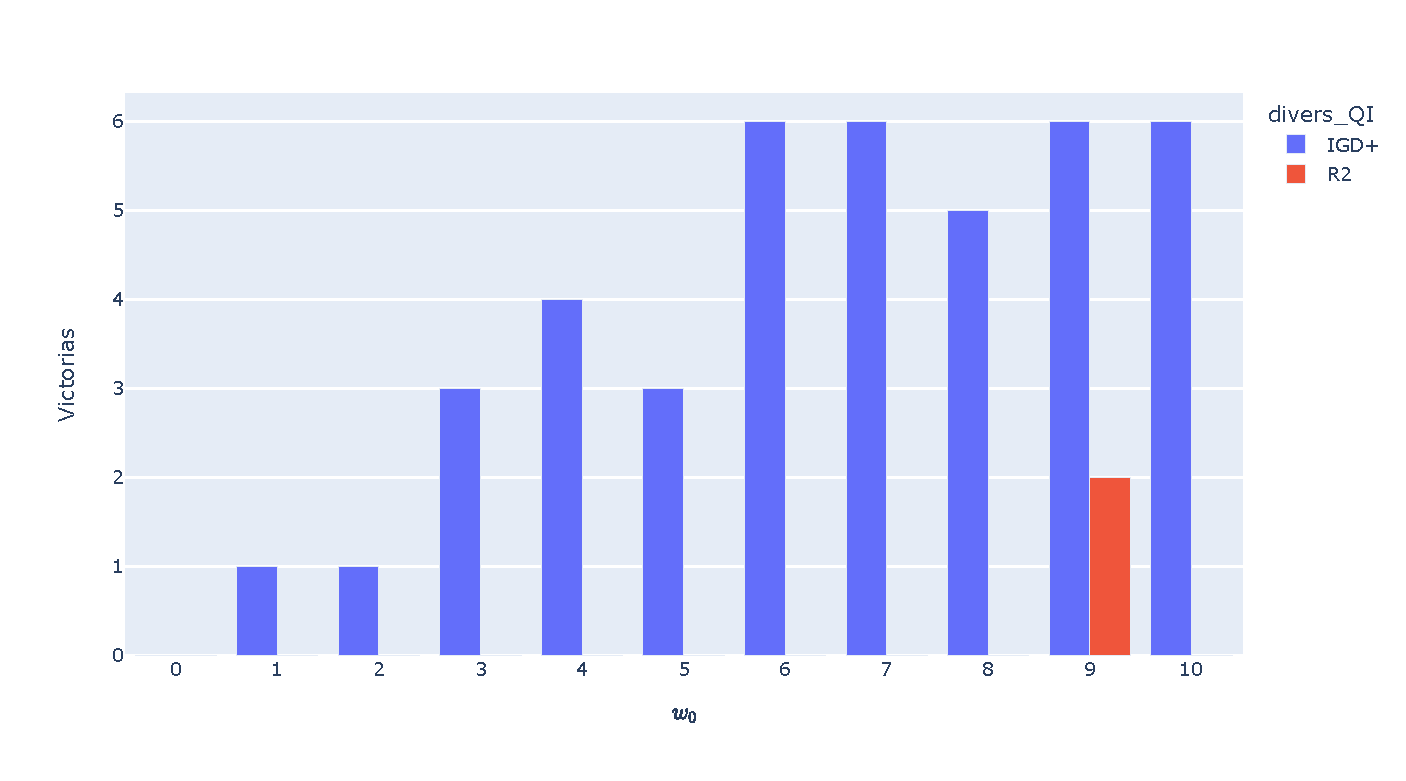
\includegraphics[width=\textwidth]{Figuras/conteo_borda_WFG4_obj3_indhv.pdf}
    \caption[Conteo de borda]{Conteo de borda de cada peso. Es útil comparar esta Figura con \ref{fig:heat}.}
    \label{fig:borda_problema}
\end{figure}

Vemos de la Figura \ref{fig:borda_problema} que a mayor peso suele haber más victorias, sin embargo, el valor de 0.7 parece haber encontrado un caso interesante en el que un mayor énfasis en la Energía-S ayuda a mejorar las victorias en un indicador de convergencia como el Hipervolumen. 

\subsection{Agregación por número de objetivos}

En esta sección se realizan agregaciones por número de objetivos de todos los conteos de borda. Es decir, estamos uniendo todos los indicadores sin importar si son de convergencia o diversidad. Las siguientes Figuras\ref{fig:borda_obj_2}, \ref{fig:borda_obj_3}, \ref{fig:borda_obj_4}, \ref{fig:borda_obj_5}, \ref{fig:borda_obj_6} y  \ref{fig:borda_obj_7} nos muestran el número de victorias promedio para cada peso. Esto es, de todos los problemas considerados para cada número de objetivos, cuánto sale el conteo de borda de un valor fijo de $w_0$. Es decir, cuántas victorias tiene con respecto a todos los otros pesos.   

\begin{figure} [H]
    \centering
    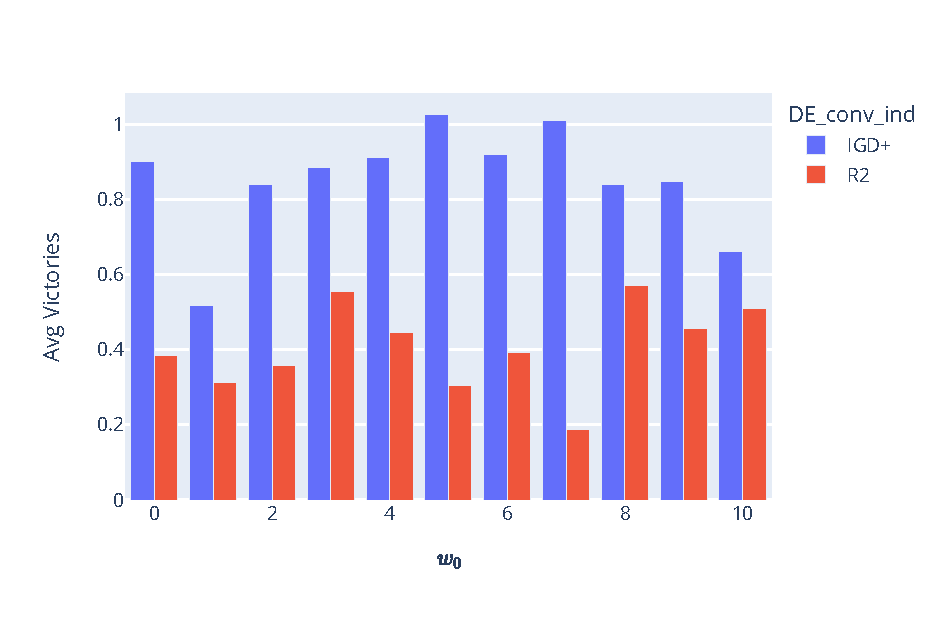
\includegraphics[width=\textwidth]{Figuras/borda_obj_2.pdf}
    \caption[Conteo de borda por número de objetivos]{Quién gana más, para todos los indicadores, conforme cambiamos el peso, para 2 objetivos.}
    \label{fig:borda_obj_2}
\end{figure}

\begin{figure} [H]
    \centering
    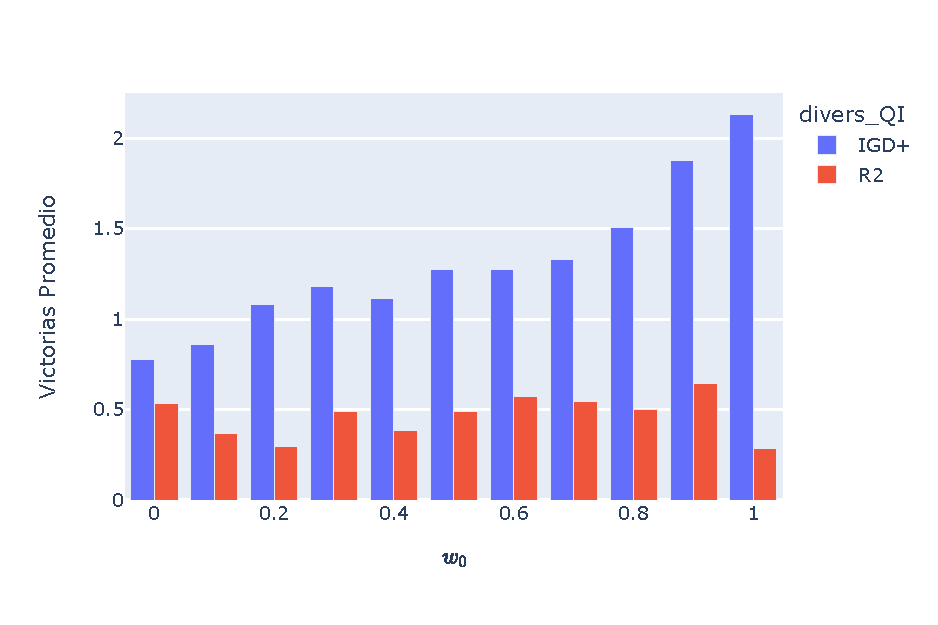
\includegraphics[width=\textwidth]{Figuras/borda_obj_3.pdf}
    \caption[Conteo de borda por número de objetivos]{Quién gana más, para todos los indicadores, conforme cambiamos el peso, para 3 objetivos.}
    \label{fig:borda_obj_3}
\end{figure}

\begin{figure} [H]
    \centering
    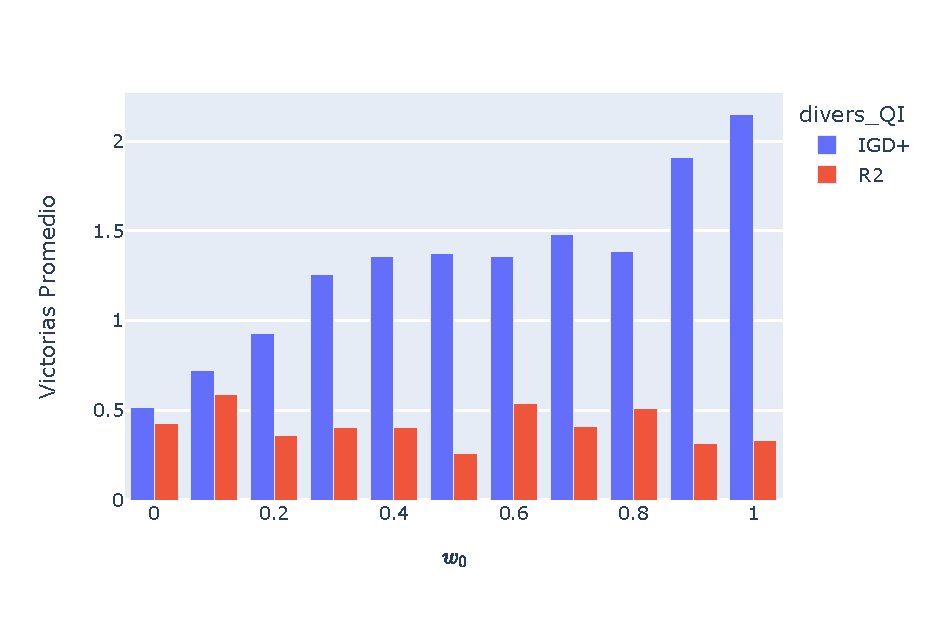
\includegraphics[width=\textwidth]{Figuras/borda_obj_4.pdf}
    \caption[Conteo de borda por número de objetivos]{Quién gana más, para todos los indicadores, conforme cambiamos el peso, para 4 objetivos.}
    \label{fig:borda_obj_4}
\end{figure}

\begin{figure} [H]
    \centering
    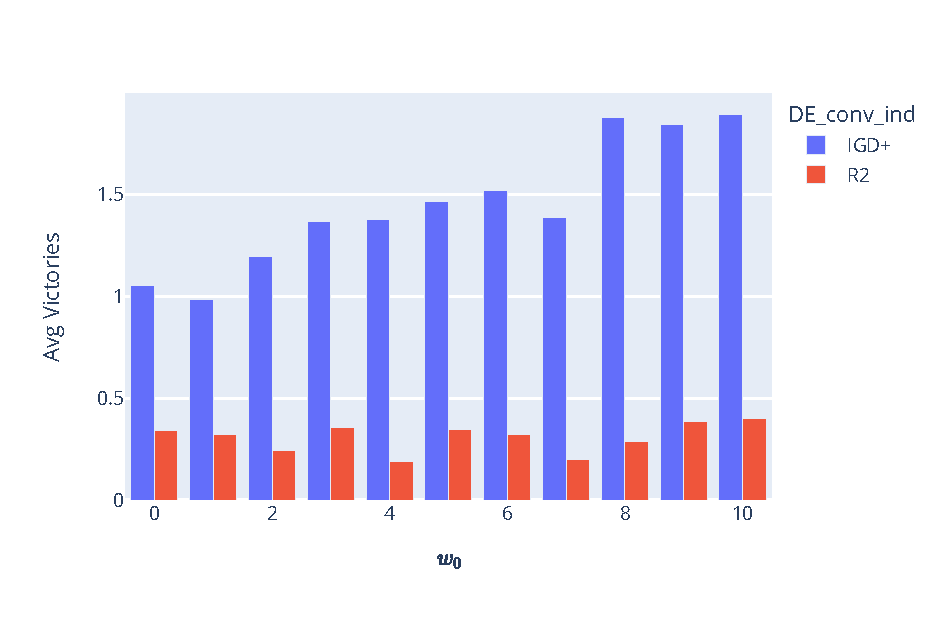
\includegraphics[width=\textwidth]{Figuras/borda_obj_5.pdf}
    \caption[Conteo de borda por número de objetivos]{Quién gana más, para todos los indicadores, conforme cambiamos el peso, para 5 objetivos.}
    \label{fig:borda_obj_5}
\end{figure}

\begin{figure} [H]
    \centering
    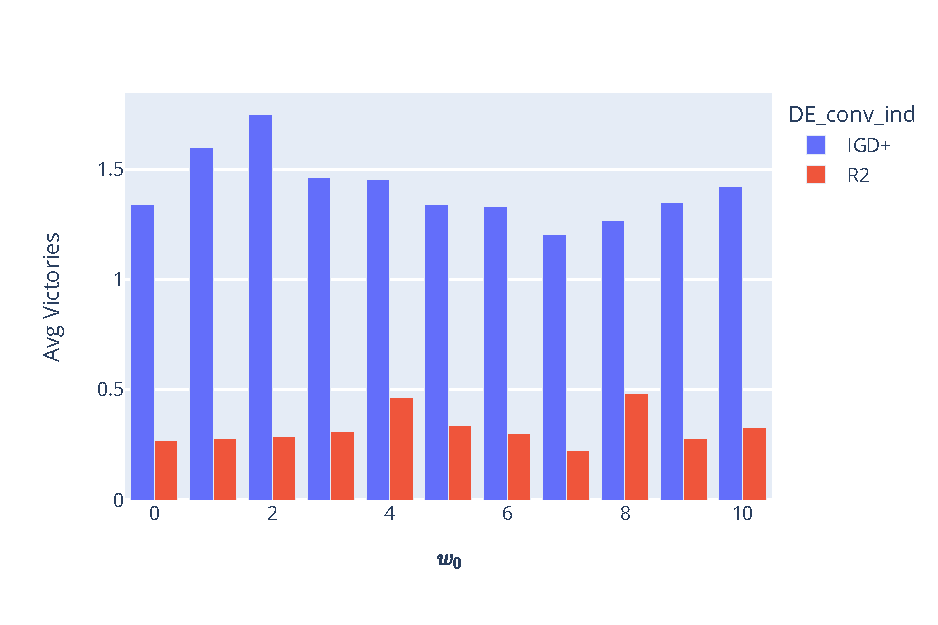
\includegraphics[width=\textwidth]{Figuras/borda_obj_6.pdf}
    \caption[Conteo de borda por número de objetivos]{Quién gana más, para todos los indicadores, conforme cambiamos el peso, para 6 objetivos.}
    \label{fig:borda_obj_6}
\end{figure}

\begin{figure} [H]
    \centering
    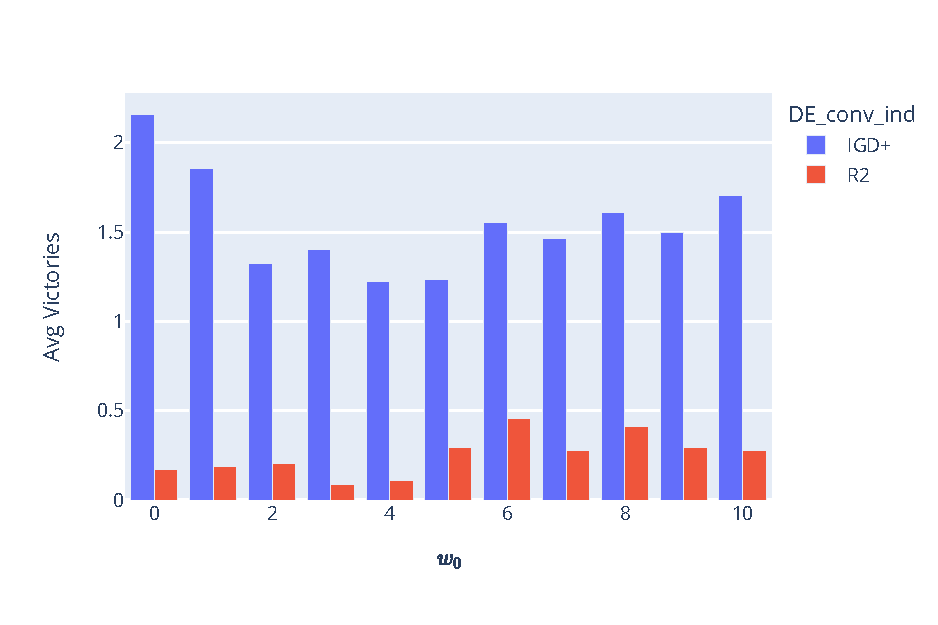
\includegraphics[width=\textwidth]{Figuras/borda_obj_7.pdf}
    \caption[Conteo de borda por número de objetivos]{Quién gana más, para todos los indicadores, conforme cambiamos el peso, para 7 objetivos.}
    \label{fig:borda_obj_7}
\end{figure}


Es importante destacar las diferencias en escala de los dos algoritmos. Claramente en todas las Figuras \ref{fig:borda_obj_2}, \ref{fig:borda_obj_3}, \ref{fig:borda_obj_4}, \ref{fig:borda_obj_5}, \ref{fig:borda_obj_6} y  \ref{fig:borda_obj_7} hay menos proporción de victorias del algoritmo de R2 y parecen no seguir ningún patrón para algún numero de objetivos. Así, la discusión que sigue se hace tomando en cuenta sólo a los valores del algoritmo de IGD+. 
Parece haber una preferencia para $w_0$ grande en dimensiones 3 a 5, notamos como las victorias van ascendiendo de forma monótona conforme le damos más peso a el IGD+ sobre la Energía-S. Sin embargo, para 2,6 y 7 no es tan claro que es mejor darle prioridad al indicador IGD+. Esto parece ir en contra de lo dicho en \cite{PFI} donde se escogió un $w_0$ mayor para mayores dimensiones bajo el suspuesto de que el indicador de diversidad podría provocar que se estancara la convergencia de la aproximación. Sin embargo, como hemos agrupado todos los indicadores esto también podría ser efecto de que los indicadores de diversidad tienden a ganar más conforme aumentamos los objetivos. Para explorar las consecuencias de este párrafo miraremos ahora una agregaciones por indicadores.

\subsection{Agregación por Indicador}

A continuación se realiza un promedio, por indicador, sobre todos los problemas de los conteos de borda para diferentes combinaciones de pesos. Para aclarar la discusión se dividirá en dos partes; en una se hablarán de los indicadores de convergencia, es decir, que tan bien converge. 



\subsection*{Conteos de Borda para Indicadores de Convergencia}

\begin{figure} [H]
    \centering
    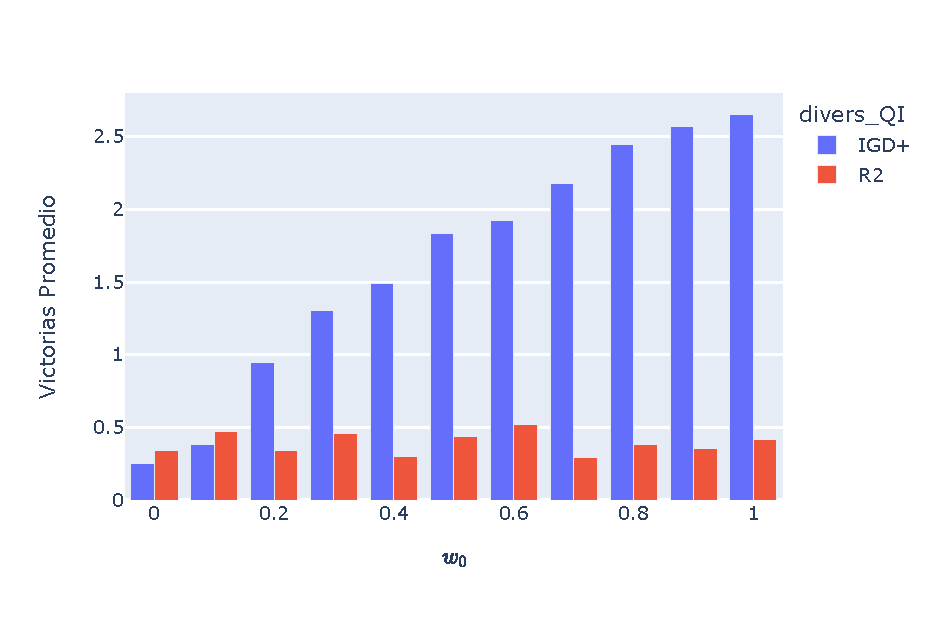
\includegraphics[width=\textwidth]{Figuras/borda_obj_ind_hv.pdf}
    \caption[Conteo de borda HV]{Victorias promedio por problema usando al indicador \textbf{HV} conforme cambiamos los pesos de $w_0$ para todas las dimensiones.}
    \label{fig:borda_hv}
\end{figure}

\begin{figure} [H]
    \centering
    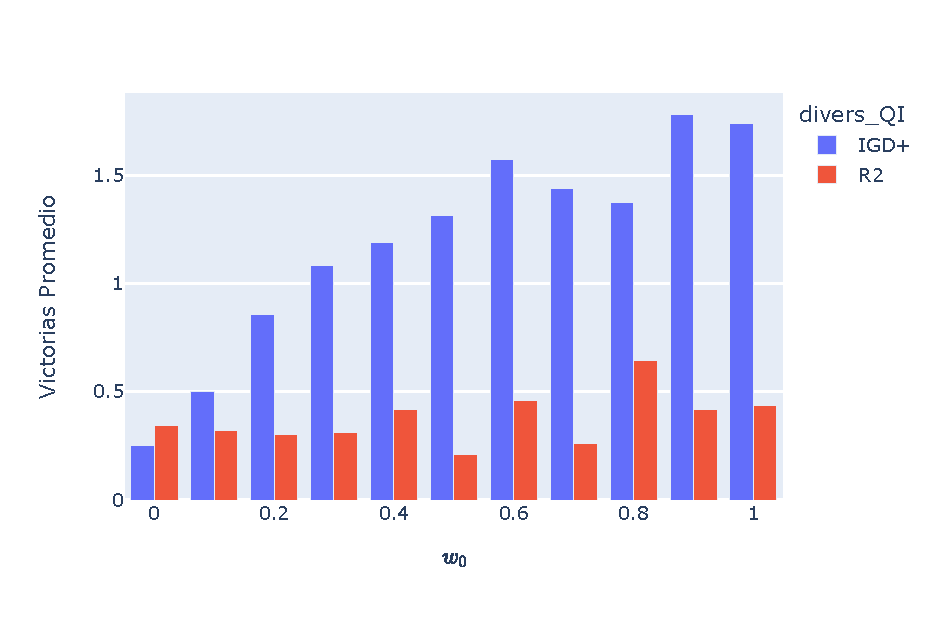
\includegraphics[width=\textwidth]{Figuras/borda_obj_ind_eps+.pdf}
    \caption[Conteo de borda Epsilon +]{Victorias promedio por problema usando al indicador \textbf{$\epsilon +$} conforme cambiamos los pesos de $w_0$ para todas las dimensiones.}
    \label{fig:borda_epsp}
\end{figure}

\begin{figure} [H]
    \centering
    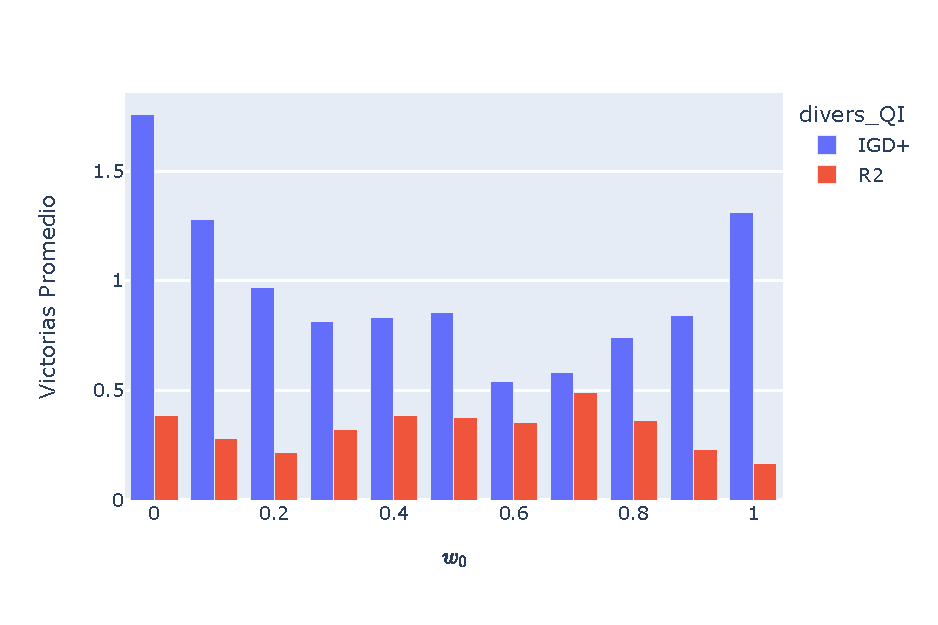
\includegraphics[width=\textwidth]{Figuras/borda_obj_ind_r2.pdf}
\caption[Conteo de borda R2]{Victorias promedio por problema usando al indicador \textbf{R2} conforme cambiamos los pesos de $w_0$ para todas las dimensiones.}
\label{fig:borda_R2}
\end{figure}

Vemos de las Figuras \ref{fig:borda_hv}, \ref{fig:borda_epsp} y \ref{fig:borda_R2} que los indicadores de convergencia que no son R2 tienen un comportamiento monotónico hacia mayores pesos de $w_0$. Es decir, al darle más peso al indicador de convergencia (ya sea IGD+ o R2) en la escalarización de Tchebycheff (Ecuación \ref{eq:ATCH}) obtenemos mayores victorias significativas. No podemos dar una conclusión satisfactoria acerca de porqué R2 tiene este comportamiento.

Ahora miraremos los de convergencia que usan un conjunto de referencia de Pareto, es decir IGD e IGD+. 

\begin{figure} [H]
    \centering
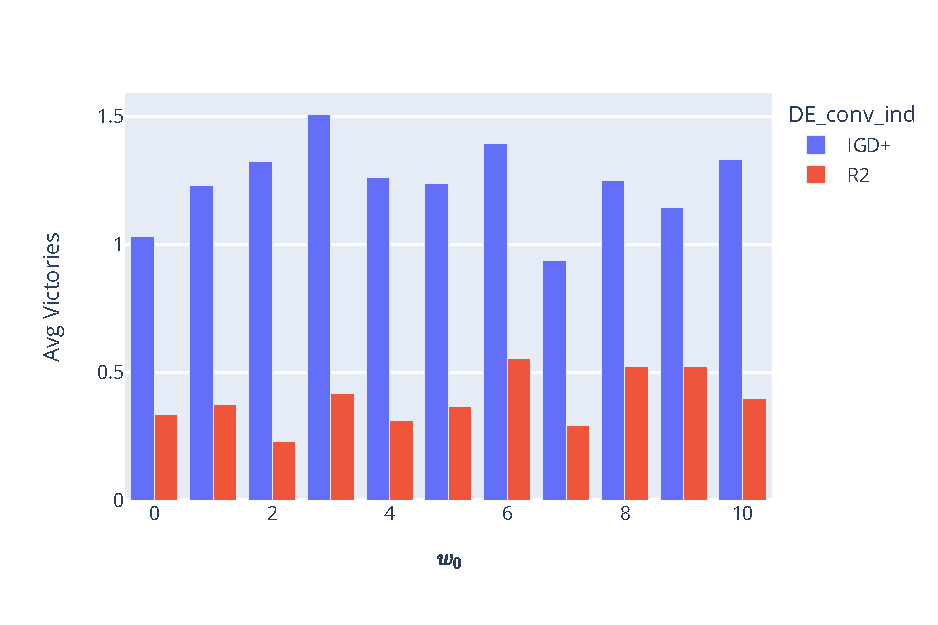
\includegraphics[width=\textwidth]{Figuras/borda_obj_ind_igd.pdf}
\caption[Conteo de borda IGD]{Victorias promedio por problema usando al indicador \textbf{IGD} conforme cambiamos los pesos de $w_0$ para todas las dimensiones.}
\label{fig:borda_igd}
\end{figure}

\begin{figure} [H]
    \centering
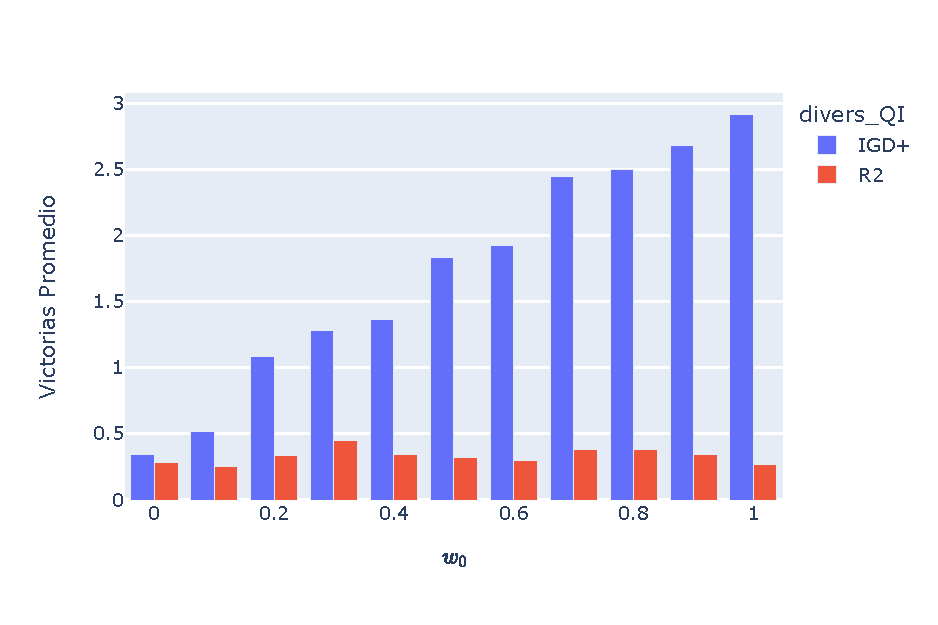
\includegraphics[width=\textwidth]{Figuras/borda_obj_ind_igd+.pdf}
\caption[Conteo de borda IGD+]{Victorias promedio por problema usando al indicador \textbf{IGD+} conforme cambiamos los pesos de $w_0$ para todas las dimensiones.}
\label{fig:borda_igdp}
\end{figure}

En el caso de IGD, vemos en la Figura \ref{fig:borda_igd} que no se observa un comportamiento monotónico de la misma forma que con R2. Para IGD+, esto se observa en la Figura \ref{fig:borda_igdp} esto se podría deber a que el indicador no es consistente de Pareto (definido en la Ecuación \ref{eq:consistente_Pareto}).


\subsection*{Conteos de Borda para Indicadores de Diversidad}

\begin{figure} [H]
    \centering
    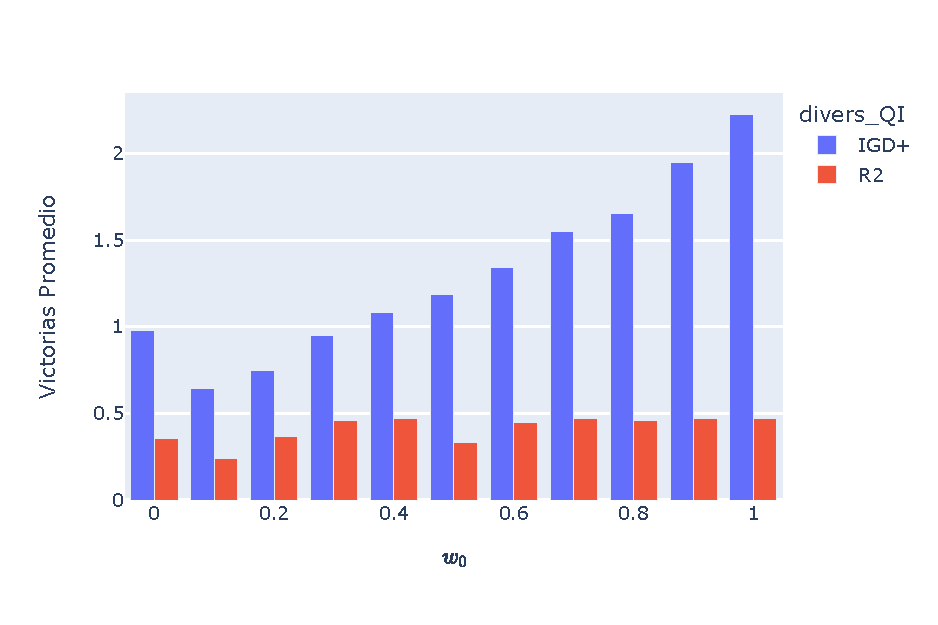
\includegraphics[width=\textwidth]{Figuras/borda_obj_ind_s-energy.pdf}
    \caption[Conteo de borda IGD+]{Victorias promedio por problema usando al indicador de \textbf{Energía-S} conforme cambiamos los pesos de $w_0$ para todas las dimensiones.}
    \label{fig:borda_senergy}
\end{figure}

\begin{figure} [H]
    \centering
    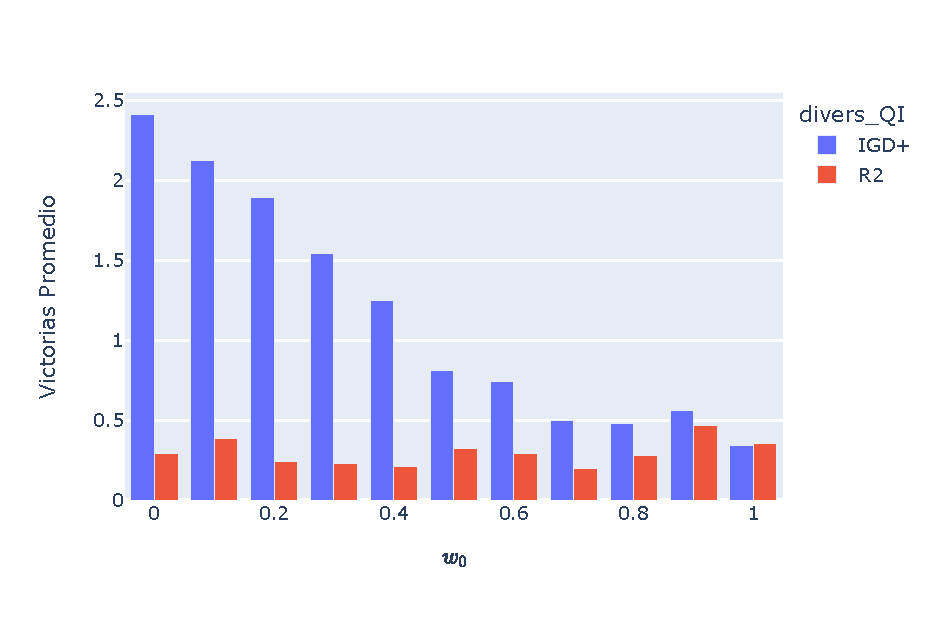
\includegraphics[width=\textwidth]{Figuras/borda_obj_ind_spd.pdf}
\caption[Conteo de borda IGD+]{Victorias promedio por problema usando al indicador \textbf{SPD} conforme cambiamos los pesos de $w_0$ para todas las dimensiones.}
\label{fig:borda_spd}
\end{figure}



Para los indicadores de diversidad, en las Figuras \ref{fig:borda_senergy} y \ref{fig:borda_spd}, vemos que tenemos el comportamiento esperado para ambos, es decir, decrece el número de victorias de forma monótona conforme aumentamos el peso al indicador de convergencia. Para R2 este ordenamiento no se mantiene para ninguno de los indicadores de diversidad y notamos que para IGD+ existe una mejora entre la combinación de pesos $w_0=(0.9,0.1)$ y la de $(0.001,0.999)$ lo que indicaría que para obtener una mejor diversidad entre estas dos elecciones conviene no maximizar la diversidad paso a paso.  

% \begin{itemize}
%     \item Mostrar diferentes visualizaciones
%     \item Tablas de cada uno de los valores de pesos. Con medias, desviaciones estándar y cuál es mejor según Wilcoxon.
%     \item Boxplots representando lo de las Tablas.
%     \item Gráfico de convergencia (número de evaluaciones (mediana) de función x, valor del indicador en esa generación y): para cada problema hay uno y por cada problema hay una línea de cada combinación de indicadores.
%     \item Conteos de borda para los rankings para ver el ganador.
%     \item Ejemplos de frentes (mediana de la última generación) para más dimensiones PCP. Proyecciones tal vez de casos interesantes. 
%     \item En el apéndice irían todos.   
% \end{itemize}




% \begin{table}[H]
%     \centering
%     \begin{tabular}{|c|c|c|c|}
%     \textbf{Problema} & \textbf{Variables objetivo} & \textbf{Variables decisión} & \textbf{Características PF}                                                                                                 \\ \hline
%     WFG1              & 2,3,4,5,6,7                 & 24,26,28,30,32,34           & \begin{tabular}[c]{@{}c@{}}separable, unifrontal \\ $f_{n_var}$ convexo, el resto mixto\end{tabular}                        \\
%     WFG2              & 2,3,4,5,6,7                 & 24,26,28,30,32,34           & \begin{tabular}[c]{@{}c@{}}No separable.\\ $f_{n_var}$ unimodal, el resto multimodal.\\ Convexo, desconectado.\end{tabular} \\
%     WFG3              & 2,3,4,5,6,7                 & 24,26,28,30,32,34           & \begin{tabular}[c]{@{}c@{}}No separable. Unifrontal.\\ Lineal, degenerado\end{tabular}                                      \\
%     WFG4              & 2,3,4,5,6,7                 & 24,26,28,30,32,34           & Separable. Multifrontal. Cóncavo.                                                                                           \\
%     WFG5              & 2,3,4,5,6,7                 & 24,26,28,30,32,34           & Separable. Deceptivo. Cóncavo.                                                                                              \\
%     WFG6              & 2,3,4,5,6,7                 & 24,26,28,30,32,34           & No separable. Unifrontal.Cóncavo.                                                                                           \\
%     WFG7              & 2,3,4,5,6,7                 & 24,26,28,30,32,34           & Separable. Unifrontal.Cóncavo.                                                                                              \\
%     WFG8              & 2,3,4,5,6,7                 & 24,26,28,30,32,34           & No separable,Unifrontal. Cóncavo                                                                                            \\
%     WFG9              & 2,3,4,5,6,7                 & 24,26,28,30,32,34           & \begin{tabular}[c]{@{}c@{}}No separable. Multifrontal, deceptivo.\\ Cóncavo\end{tabular}                                   
%     \end{tabular}
% \end{table}
% \begin{table}[H]
%     \centering
%     \begin{tabular}{|c|c|c|c|}
%     \textbf{Problema} & \textbf{Variables objetivo} & \textbf{Variables decisión} & \textbf{Características PF}                                                                                                                                   \\ \hline
%     DTLZ1             & 2,3,4,5,6,7                 & 6,7,8,9,10,11               & separable, multifrontal, lineal                                                                                                                               \\
%     DTLZ2             & 2,3,4,5,6,7                 & 12,13,14,15,16              & separable, unifrontal, cóncavo                                                                                                                                \\
%     DTLZ3             & 2,3,4,5,6,7                 & 12,13,14,15,16              & separable, multifrontal, cóncavo                                                                                                                              \\
%     DTLZ4             & 2,3,4,5,6,7                 & 12,13,14,15,16              & separable, unifrontal, cóncavo                                                                                                                                \\
%     DTLZ5             & 2,3,4,5,6,7                 & 12,13,14,15,16              & \begin{tabular}[c]{@{}c@{}}unifrontal, \\ degenerado\end{tabular}                                                                                             \\
%     DTLZ6             & 2,3,4,5,6,7                 & 12,13,14,15,16              & unifrontal, degenerado                                                                                                                                        \\
%     DTLZ7             & 2,3,4,5,6,7                 & 21,22,23,24,25,26           & \begin{tabular}[c]{@{}c@{}}$f_{n_var}$ separable, para el resto no aplica\\ $f_{n_var}$ unimodal, para el resto multimodal\\ desconectado, mixto\end{tabular}
%     \end{tabular}
%     \caption[Problemas prueba usados ]{Problemas pruebas usados así como sus variables objetivo, de decisión,  y algunas características de su frente de Pareto.}
%     \label{Tabla:problema_prueba}
% \end{table}
